% Template for PLoS
% Version 3.5 March 2018
%
% % % % % % % % % % % % % % % % % % % % % %
%
% -- IMPORTANT NOTE
%
% This template contains comments intended 
% to minimize problems and delays during our production 
% process. Please follow the template instructions
% whenever possible.
%
% % % % % % % % % % % % % % % % % % % % % % % 
%
% Once your paper is accepted for publication, 
% PLEASE REMOVE ALL TRACKED CHANGES in this file 
% and leave only the final text of your manuscript. 
% PLOS recommends the use of latexdiff to track changes during review, as this will help to maintain a clean tex file.
% Visit https://www.ctan.org/pkg/latexdiff?lang=en for info or contact us at latex@plos.org.
%
%
% There are no restrictions on package use within the LaTeX files except that 
% no packages listed in the template may be deleted.
%
% Please do not include colors or graphics in the text.
%
% The manuscript LaTeX source should be contained within a single file (do not use \input, \externaldocument, or similar commands).
%
% % % % % % % % % % % % % % % % % % % % % % %
%
% -- FIGURES AND TABLES
%
% Please include tables/figure captions directly after the paragraph where they are first cited in the text.
%
% DO NOT INCLUDE GRAPHICS IN YOUR MANUSCRIPT
% - Figures should be uploaded separately from your manuscript file. 
% - Figures generated using LaTeX should be extracted and removed from the PDF before submission. 
% - Figures containing multiple panels/subfigures must be combined into one image file before submission.
% For figure citations, please use "Fig" instead of "Figure".
% See http://journals.plos.org/plosone/s/figures for PLOS figure guidelines.
%
% Tables should be cell-based and may not contain:
% - spacing/line breaks within cells to alter layout or alignment
% - do not nest tabular environments (no tabular environments within tabular environments)
% - no graphics or colored text (cell background color/shading OK)
% See http://journals.plos.org/plosone/s/tables for table guidelines.
%
% For tables that exceed the width of the text column, use the adjustwidth environment as illustrated in the example table in text below.
%
% % % % % % % % % % % % % % % % % % % % % % % %
%
% -- EQUATIONS, MATH SYMBOLS, SUBSCRIPTS, AND SUPERSCRIPTS
%
% IMPORTANT
% Below are a few tips to help format your equations and other special characters according to our specifications. For more tips to help reduce the possibility of formatting errors during conversion, please see our LaTeX guidelines at http://journals.plos.org/plosone/s/latex
%
% For inline equations, please be sure to include all portions of an equation in the math environment.  For example, x$^2$ is incorrect; this should be formatted as $x^2$ (or $\mathrm{x}^2$ if the romanized font is desired).
%
% Do not include text that is not math in the math environment. For example, CO2 should be written as CO\textsubscript{2} instead of CO$_2$.
%
% Please add line breaks to long display equations when possible in order to fit size of the column. 
%
% For inline equations, please do not include punctuation (commas, etc) within the math environment unless this is part of the equation.
%
% When adding superscript or subscripts outside of brackets/braces, please group using {}.  For example, change "[U(D,E,\gamma)]^2" to "{[U(D,E,\gamma)]}^2". 
%
% Do not use \cal for caligraphic font.  Instead, use \mathcal{}
%
% % % % % % % % % % % % % % % % % % % % % % % % 
%
% Please contact latex@plos.org with any questions.
%
% % % % % % % % % % % % % % % % % % % % % % % %

\documentclass[10pt,letterpaper]{article}
\usepackage[top=0.85in,left=2.75in,footskip=0.75in]{geometry}

% amsmath and amssymb packages, useful for mathematical formulas and symbols
\usepackage{amsmath,amssymb}

\DeclareMathOperator{\atantwo}{atan2}
\DeclareMathOperator{\arctantwo}{arctan2}
\DeclareMathOperator*{\argmax}{argmax} % thin space, limits underneath in displays
\usepackage{diagbox}

% Use adjustwidth environment to exceed column width (see example table in text)
\usepackage{changepage}

% Use Unicode characters when possible
\usepackage[utf8x]{inputenc}

% textcomp package and marvosym package for additional characters
\usepackage{textcomp,marvosym}

% cite package, to clean up citations in the main text. Do not remove.
\usepackage{cite}

% Use nameref to cite supporting information files (see Supporting Information section for more info)
\usepackage{nameref,hyperref}

% line numbers
\usepackage[right]{lineno}

% ligatures disabled
\usepackage{microtype}
\DisableLigatures[f]{encoding = *, family = * }

% color can be used to apply background shading to table cells only
\usepackage[table]{xcolor}

% array package and thick rules for tables
\usepackage{array}

% create "+" rule type for thick vertical lines
\newcolumntype{+}{!{\vrule width 2pt}}

% create \thickcline for thick horizontal lines of variable length
\newlength\savedwidth
\newcommand\thickcline[1]{%
	\noalign{\global\savedwidth\arrayrulewidth\global\arrayrulewidth 2pt}%
	\cline{#1}%
	\noalign{\vskip\arrayrulewidth}%
	\noalign{\global\arrayrulewidth\savedwidth}%
}

% \thickhline command for thick horizontal lines that span the table
\newcommand\thickhline{\noalign{\global\savedwidth\arrayrulewidth\global\arrayrulewidth 2pt}%
	\hline
	\noalign{\global\arrayrulewidth\savedwidth}}


% Remove comment for double spacing
%\usepackage{setspace} 
%\doublespacing

% Text layout
\raggedright
\setlength{\parindent}{0.5cm}
\textwidth 5.25in 
\textheight 8.75in

% Bold the 'Figure #' in the caption and separate it from the title/caption with a period
% Captions will be left justified
\usepackage[aboveskip=1pt,labelfont=bf,labelsep=period,justification=raggedright,singlelinecheck=off]{caption}
\renewcommand{\figurename}{Fig}

% Use the PLoS provided BiBTeX style
\bibliographystyle{plos2015}

% Remove brackets from numbering in List of References
\makeatletter
\renewcommand{\@biblabel}[1]{\quad#1.}
\makeatother



% Header and Footer with logo
\usepackage{lastpage,fancyhdr,graphicx}
\usepackage{epstopdf}
%\pagestyle{myheadings}
\pagestyle{fancy}
\fancyhf{}
%\setlength{\headheight}{27.023pt}
%\lhead{\includegraphics[width=2.0in]{PLOS-submission.eps}}
\rfoot{\thepage/\pageref{LastPage}}
\renewcommand{\headrulewidth}{0pt}
\renewcommand{\footrule}{\hrule height 2pt \vspace{2mm}}
\fancyheadoffset[L]{2.25in}
\fancyfootoffset[L]{2.25in}
\lfoot{\today}

%% Include all macros below

\newcommand{\lorem}{{\bf LOREM}}
\newcommand{\ipsum}{{\bf IPSUM}}

%% END MACROS SECTION


\begin{document}
	\vspace*{0.2in}
	
	% Title must be 250 characters or less.
	\begin{flushleft}
		{\Large
			\textbf\newline{Sleep Monitoring with Portable Wi-Fi} % Please use "sentence case" for title and headings (capitalize only the first word in a title (or heading), the first word in a subtitle (or subheading), and any proper nouns).
		}
		\newline
		% Insert author names, affiliations and corresponding author email (do not include titles, positions, or degrees).
		\\
		Name1 Surname\textsuperscript{1,2\Yinyang},
		Name2 Surname\textsuperscript{2\Yinyang},
		Name3 Surname\textsuperscript{2,3\textcurrency},
		Name4 Surname\textsuperscript{2},
		Name5 Surname\textsuperscript{2\ddag},
		Name6 Surname\textsuperscript{2\ddag},
		Name7 Surname\textsuperscript{1,2,3*},
		with the Lorem Ipsum Consortium\textsuperscript{\textpilcrow}
		\\
		\bigskip
		\textbf{1} Affiliation Dept/Program/Center, Institution Name, City, State, Country
		\\
		\textbf{2} Affiliation Dept/Program/Center, Institution Name, City, State, Country
		\\
		\textbf{3} Affiliation Dept/Program/Center, Institution Name, City, State, Country
		\\
		\bigskip
		
		% Insert additional author notes using the symbols described below. Insert symbol callouts after author names as necessary.
		% 
		% Remove or comment out the author notes below if they aren't used.
		%
		% Primary Equal Contribution Note
		\Yinyang These authors contributed equally to this work.
		
		% Additional Equal Contribution Note
		% Also use this double-dagger symbol for special authorship notes, such as senior authorship.
		\ddag These authors also contributed equally to this work.
		
		% Current address notes
		\textcurrency Current Address: Dept/Program/Center, Institution Name, City, State, Country % change symbol to "\textcurrency a" if more than one current address note
		% \textcurrency b Insert second current address 
		% \textcurrency c Insert third current address
		
		% Deceased author note
		\dag Deceased
		
		% Group/Consortium Author Note
		\textpilcrow Membership list can be found in the Acknowledgments section.
		
		% Use the asterisk to denote corresponding authorship and provide email address in note below.
		* correspondingauthor@institute.edu
		
	\end{flushleft}
	% Please keep the abstract below 300 words
	\section*{Abstract}
	
	\iffalse
	\fi
	WiFi human sensing is being challenged by researchers continuously e.g. Activity Classification, Localization and etc. However, we believed WiFi can do more. In this paper, we paired WiFi transmitting pattern to human sleep stage to create a mapping rule of those. we used ESP32 which is a reachable single board computer and strengthened its WiFi signal with 2 directional external antennae. After gathering WiFi variation with Sleep Stage from a sleep tracker, we applied machine learning to merge them. We used Long-short term memory (LSTM) to the framework since we know pattern of moving matters to Sleep Stage. So, we are to map a sleeping stage to a sequence of WiFi snapshots instead of one-to-one like others which makes this called ``Sleep monitoring''. we tested with newly collected data sizing more than 6,000 frames of sequences. To evaluate the result, we compared annotated Sleep Stage with predicted Sleep Stage and summarized their accuracy which finally resulted as that it is possible to classify 4 human sleep stages from WiFi in ESP32.
	
	
	
	\linenumbers
	
	% Use "Eq" instead of "Equation" for equation citations.
	\section*{Introduction}
	Wi-Fi is one of the most common network mediums nowadays. Pervasively, it is used for establishing a wireless network to connect to the internet. But, there are still many more functions Wi-Fi is good at. Wi-Fi can also be applied in fields beside connecting to the internet according to its stability being upgraded continuously. Decent Wi-Fi connectivity can extract more data other than the data to be transmitted like concentration, speed, obstacle between the transmission. Those can be composed to be many useful applications like Localization, Activity Classification and etc.
	
	In order to achieve the applications like mentioned, There are many works tried to extract deep features from Wi-Fi. But, they are mostly working with very specific tools and Network Interface Card (NIC) connected to a laptop running Linux that is currently one of the ways allowing to obtain fine-grain Channel State Information (CSI), the descriptive data of the  Wi-Fi propagating in that environment. Those limitations significantly decrease simplicity of implementation. It is hard for public demonstration and integration with many updated tools.
	
	Actually, there are other existing ways for obtaining the CSI. One is from a ubiquitously used microprocessor, ESP32. which is still not much explored in Wi-Fi exploiting field. It is simple to implement and can be easily integrated with other tools in many platforms due to its massively produced external tools. 
	
	
	Human sleep stage monitoring is being observed for a whlie and recently applied on commercial products. As sleeping is significant to all persons and can lead to many serious deceases, people are more concerned on utilizing their sleepness with using devices those are able to inform them their sleep information e.g. smartwatches, smart mattress, smart rings and etc.
	But, those devices are considerably affect sleepness since it needs a contact to users' bodies. 
	
	So, this paper proposes a contactless sleep monitoring with Wi-Fi CSI from ESP32 where users can applied with easy-to-find microprocessor and monitor their sleep stage without contacting to their bodies.
	This allows sleep monitoring to be practical for other researchers and those who want to utilize their sleepness.
	
	
	
	\section*{Background}
	
	\subsection*{Human sleep stage monitoring}
	Human sleep stage monitoring is widely used as stated above. There are many types of staging. But most common and what we chose are stages of 4 which are Wake, REM (Rapid Eye Movement),  Light Sleep (Light) and Deep Sleep (Deep). Many commercial devices can log such information in time sequence. We use {Fitbit}, a popular sleep tracker watch, as our ground truth as it is a device with the most accuracy at Sleep Stage Estimation among others (ref). The {Fitbit}  can log stages with resolution of 30 seconds so, we consider a single Sleep Stage with a sequence of 30-second CSI data from Wi-Fi.
	
	
	\subsection*{Wi-Fi}\label{wifi}
	
	Wi-Fi is a well-known connectivity with no wire needed (wireless). It has been used as a medium for connecting to the internet for over 10 years. However, the Wi-Fi is the name covering IEEE 802.11 n/g/ac protocols. It delivers data through 2.4/5GHz frequency with multiple channels. The bandwidth in each channel is 22MHz. the data are to be transmitted  parallelly with multiplexing technique named orthogonal frequency division multiplexing (OFDM). Each carrier may propagate to a receiver with encountering many obstacles. The effect of that situation is the Doppler Effect.
	So, Channel State Information (CSI) is represented as physical layer indicator that can be used to investigate how each channel propagate to the receiver or back to the transmitter.
	
	If a sender sends data to a receiver through Wi-Fi, the data will be almostly not transmitted without any interference.
	
	
	
	\subsection*{CSI data}\label{CSI}
	As mentioned in \nameref{wifi} that data propagating to the receiver while touching surrounding environment, the CSI is a variation of the data. The CSI can  be found at both sender and receiver since receiver may transmit data back. Let the sender use the modulation method of 16-quadrature amplitude modulation (16-QAM) which one carrier can carry 4 bits. When the sender needs to send a `1111', the modulation returns $x=1+1i$. Then, transmit to the receiver. At the receiver, let the obtained data is $y=0.8+0.9i$. So, the CSI can be computed by the variation $h=y/x=0.2+3.4i$.
	
	Human body is literally water which reflect radio wave like Wi-Fi. \cite{wangF}, \cite{liuJ} and \cite{chowdhuryTZ} have proven that human body can affect the CSI.
	
	\subsubsection*{ESP32}\label{ESP32}
	ESP32 is a very popular single-board computer (SBC). With its affordable price and many available additional tools, ESP32 is commonly used in Internet of Things field.  Quantitative CSI can be obtained from Wi-Fi in ESP32 according to \cite{atifM}. The number of available subcarriers in ESP32 is 64.
	
	According to the detail about Wi-Fi mentioned in \nameref{wifi}, the Wi-Fi in ESP32 has some limitation. It supports only 2.4GHz frequency and can be set only one channel over a connection. The bandwidth of each channel is 22MHz. The CSI can be both obtain from Access point (AP) and Station (STA) as shown in Fig.~\ref{fig:ESP32CSI01}.  In this paper, we consider to mainly use CSI at the AP.
	The frequency of each channel is as 802.11 standard.
	
	
	
	\begin{figure}[htbp]
		
		\centerline{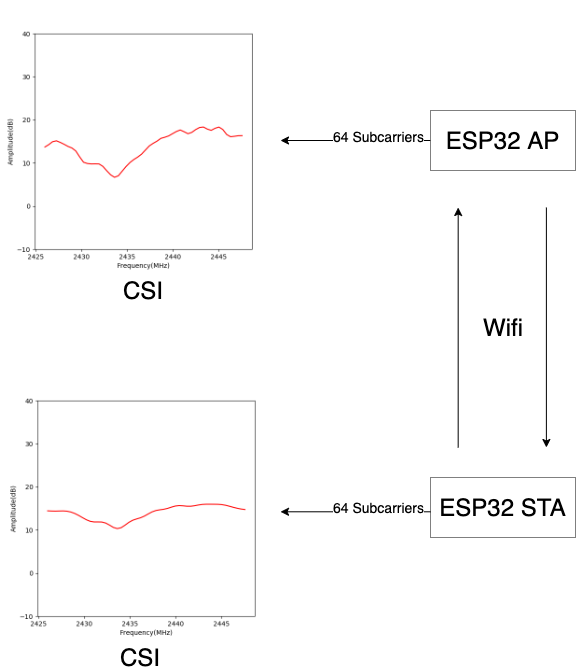
\includegraphics[width=70mm,scale=0.5]{ESP32CSI01.png}}
		\caption{CSI from ESP32s with channel 6.}
		\label{fig:ESP32CSI01}
	\end{figure}
	
	\iffalse
	\subsubsection*{Faraday cage}
	Faraday cage is invented by Michael Faraday in 1836. It is an enclosure to block electromagnetic fields. It is made of conducting material which can affect any radio frequency (e.g. Wi-Fi) to be unable to pass through.
	\fi
	
	\section*{Materials and methods}
	
	\subsection*{Concept}
	\label{concept}
	
	\begin{figure}[htbp]
		
		\centerline{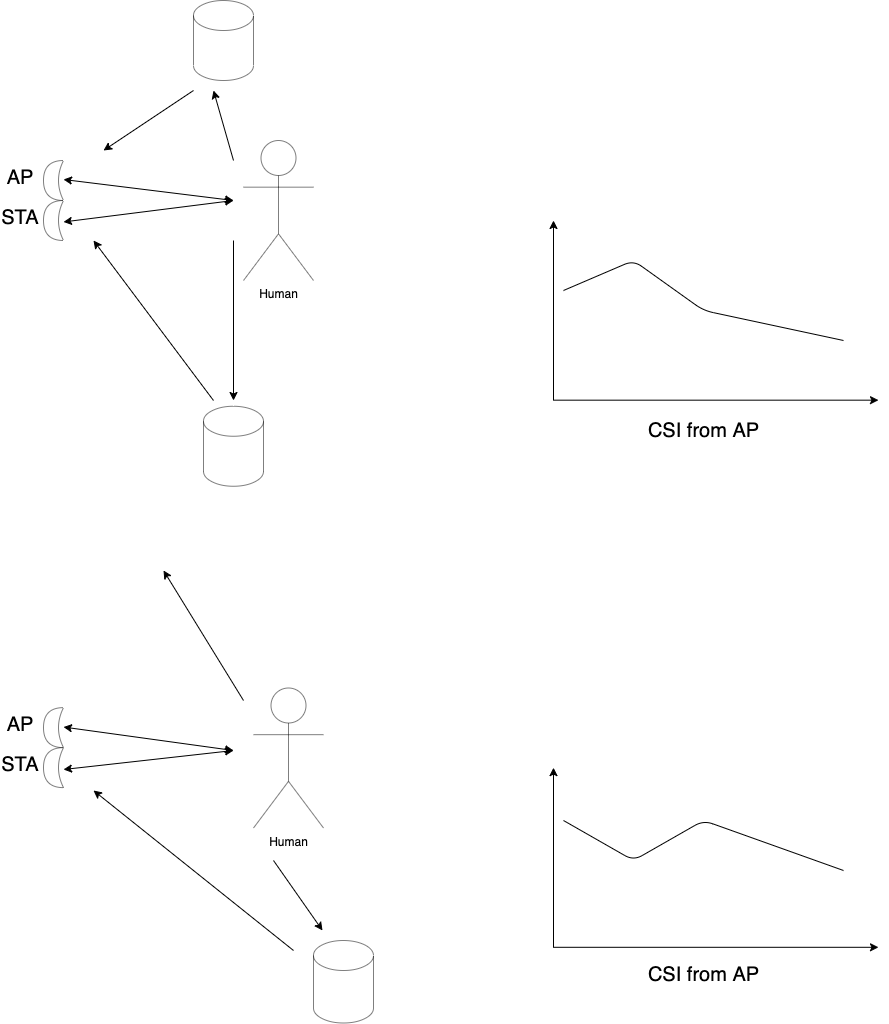
\includegraphics[width=85mm,scale=0.5]{ESP32CSI03.png}}
		\caption{2 different CSIs resulted from corresponding human poses.}
		\label{fig:ESP32CSI02}
	\end{figure}
	
	Other famous proposed works like \cite{wangF} \cite{liuJ} and \cite{hernandezSM} use omnidirectional antennas while our work uses 2 directional Wi-Fi antennae facing toward human in order to enhance thier precision as shown in Fig.~\ref{fig:SETUP01}.
	
	
	The CSI is not only affected by human body but mainly by overall environment. This means that 2 identical human poses can result obviously different CSIs if the environment around are not exactly the same as shown in Fig.~\ref{fig:ESP32CSI02}.
	
	So, the definite detection of human standing still in every environment is nearly impossible since the CSI of that situation may be found exactly matched to a CSI of the environment that a big bottle of water placed in front of ESP32.
	In short, CSI is suitable for moving target since we can focus on its change. The example of mapping CSI's change to Activity Classification can be found in \cite{chowdhuryTZ} and \cite{zouH}. Our work does likewise but focusing on Sleep Stage Monitoring instead of Activity Classification.
	
	In different environment, the CSIs are different. But, the corresponding changing of Sleep Stage may affect to the same changing pattern of CSI. This hypothesis is investigated in the upcoming parts.
	
	All steps of training and testing method are shown in Fig.~\ref{fig:TRAINSTEP} and Fig.~\ref{fig:TESTSTEP} respectively. 
	
	
	\begin{figure}[htbp]
		\centerline{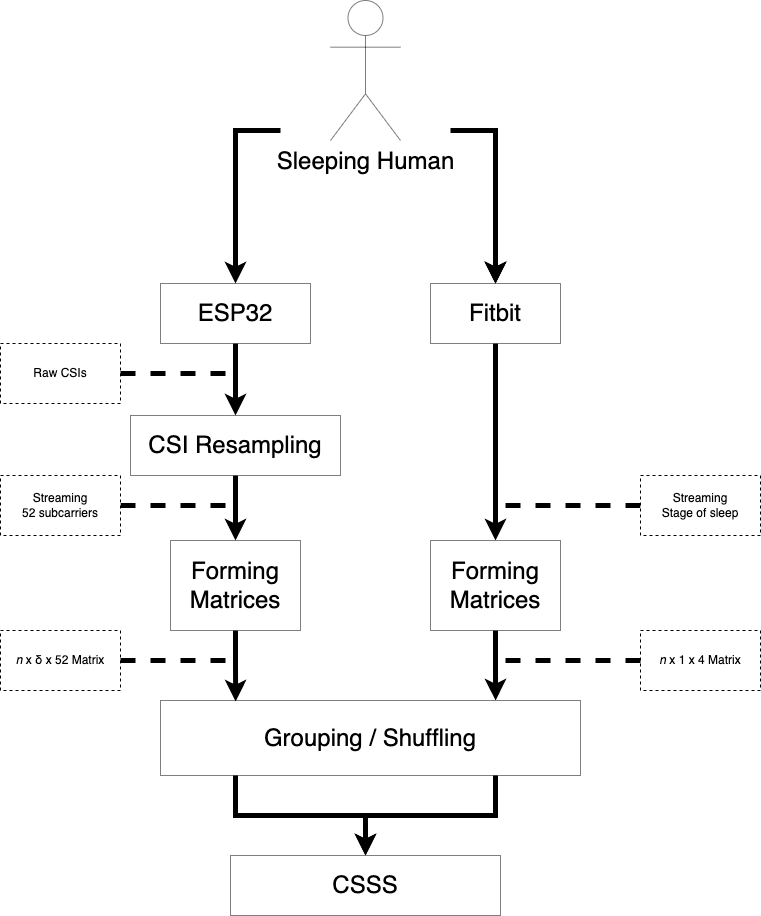
\includegraphics[width=70mm,scale=0.2]{TRAINSTEP08.png}}
		\caption{All steps of training method.}
		\label{fig:TRAINSTEP}
	\end{figure}
	\begin{figure}[htbp]
		\centerline{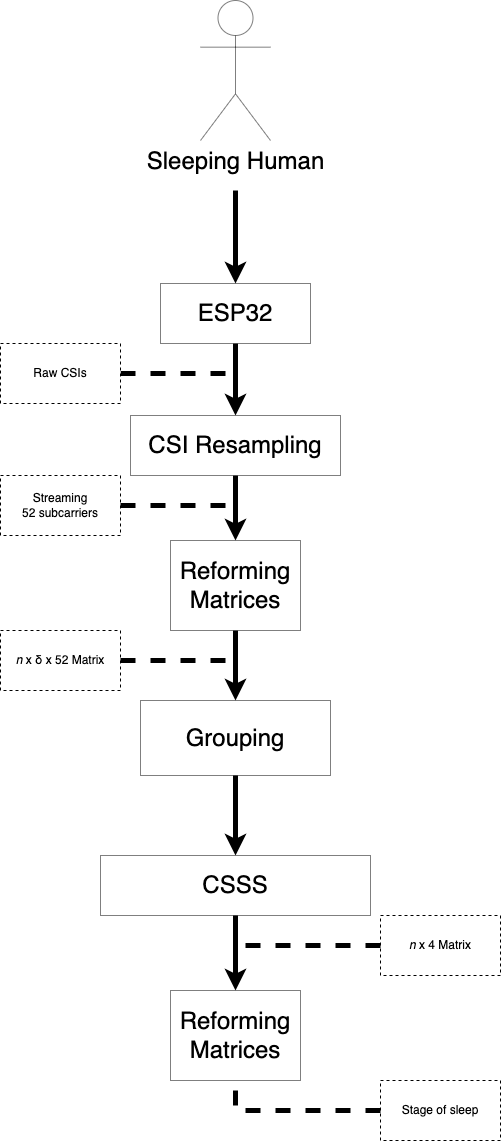
\includegraphics[width=60mm,scale=0.2]{TESTSTEP08.png}}
		\caption{All steps of testing method.}
		\label{fig:TESTSTEP}
	\end{figure}
	
	\subsection*{Training}
	
	\subsubsection*{CSI Resampling}
	
	As mentioned in \nameref{ESP32}, there are 64 subcarriers in CSI data from ESP32 but there are only 52 those are usable while the rest are null. So, we can construst a tensor of $1 \times 52$ to represent each CSI. We are to map CSI from the ESP32 to human sleep stage from {(Fitbit)}. The sampling rate of the sleep stage are locked at 30 seconds 
	since the device's limitation. So, we have one sleep stage annotations for 30 seconds. For the ESP32, the sampling rate is originally unpredictable and not constant but it is running around 70Hz. So, we do a process called ``Resampling" to the CSI data in order to maintain the dimension of each sequence. The CSI data can be resampled into any size so, we determine it as one of the parameter.
	
	An example of CSI Resampling is shown in Fig.~\ref{fig:CSIResampling01}. The top graph shows that the the original CSI is logged unstably. The bottom one is to recreate a CSI data at rate 30Hz by calculating each with 2 data at the closet timestamps from the original with a simple mathematical weight equation as in Eq.~\ref{eq:CSIResampling01} in order to recreate a CSI data with fixed identical size for all sequences.
	
	\begin{equation}
		\begin{aligned}
			& CSI_{now} = CSI_{before} \\ 
			& + \left(  \frac{ts_{now}-ts_{before}}{ts_{after}-ts_{before}}  \times (CSI_{after}-CSI_{before})   \right),
			\label{eq:CSIResampling01}
		\end{aligned}
	\end{equation}
	where $ts_{now}$, $ts_{before}$, $ts_{after}$ are desired timestamp, timestamp at the closest CSI before the desired timestamp and timestamp at the closest CSI after the desired timestamp respectively. And, $CSI_{now}$, $CSI_{before}$, $CSI_{after}$ are CSI at the desired timestamp, CSI before the desired timestamp and CSI after the desired timestamp respectively.
	
	\begin{figure}[htbp]
		\centerline{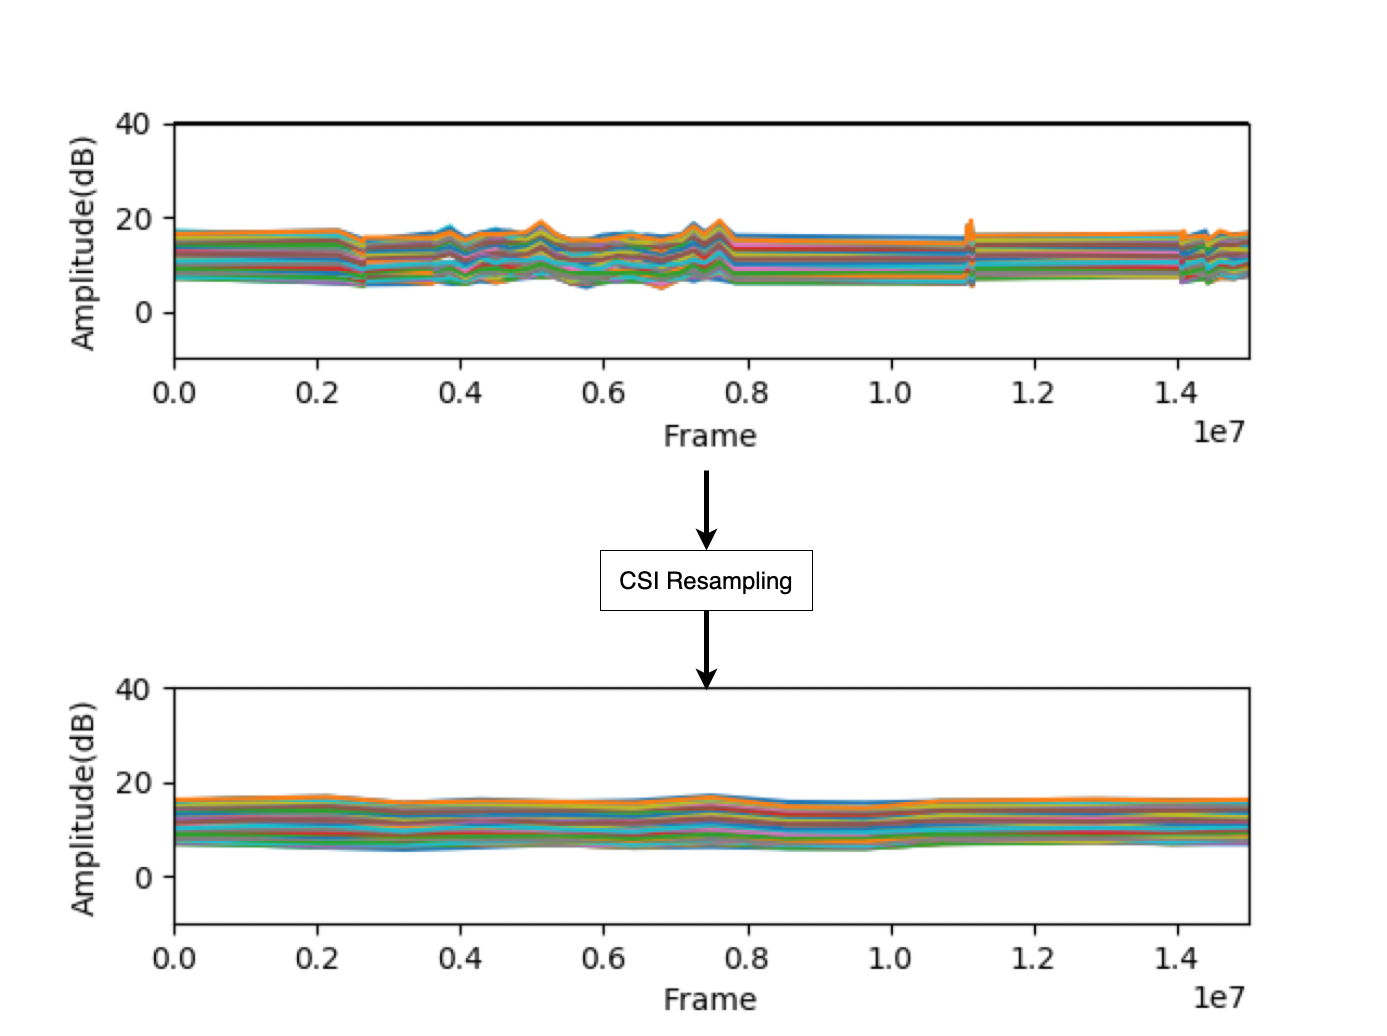
\includegraphics[width=70mm,scale=0.5]{CSIResampling03.png}}
		\caption{An example of CSI resampling.}
		\label{fig:CSIResampling01}
	\end{figure}
	
	Thus, we are able to map each CSI sequence of 30 seconds to each Sleep Stage annotation.		
	
	
	
	\subsubsection*{Data Preparation}
	Let $D$ be a set of synchronized CSI sequences and Sleep Stage package. Each pair has corresponding timestamp.
	
	
	
	\begin{equation}
		D =  {(C_t, S_t), t \in [1, n]},
		\label{eq:Dataset}
	\end{equation} where  $n$ is a number of pairs, $t$ is a timestamp, $C_t$ is a sequence of CSI data which is collected between $t-30$ to $t$ and $S_t$ is a Sleep Stage annotation as the ground truth which are collected at $t$.
	
	All $C$s has the same dimension since they are all resampled  beforehand. Let $\delta$ be the length of each $C$.
	\iffalse
	\fi
	
	\subsubsection*{Forming Matrices}
	To make the CSI and Sleep Stage data valid to the training model, they are to be formed in to a sequence of matrices.
	
	\paragraph{CSI data}
	For CSI data (left part in Fig.~\ref{fig:TRAINSTEP}), the streaming data is cut into a serie of $n \times \delta \times 52$ matrices.
	
	However, original CSI data is complex number so, we can either convert it into phase or amplitude. As mentioned in \ref{CSI}, the CSI is originally in form $h=y/x=v+wi$ so, they are parsed. For amplitude,  $\sqrt{ v^2+w^2 }$ and $\arctantwo(v, 2 )$ for phase.
	In the paper, we use amplitude.
	
	\begin{equation}
		amp =  {  \sqrt{ v_{sc}^2+w_{sc}^2 } , sc \in [1, 52]}
		\label{eq:CSIampParser}
	\end{equation}
	and
	\begin{equation}
		C =  [amp_1,...,amp_{\delta}].
		\label{eq:CSIseq}
	\end{equation}
	
	The serie length is $n$ so, a single matrix of  $n \times \delta \times 52$ is for the CSI data side.
	
	\paragraph{Sleep Stage data}
	For Sleep Stage data (right part in Fig.~\ref{fig:TRAINSTEP}), the streaming data is cut into a serie of  $n$ length resulting a single matrix of  $n \times 1$. Furthermore, each is mapped into a $1 \times 4$ weight matrix as follows.
	
	\begin{equation}
		S = \begin{cases}
			[1,0,0,0] &\text{,if sleep stage is Wake}\\
			[0,1,0,0] &\text{,if sleep stage is REM}\\
			[0,0,1,0] &\text{,if sleep stage is Light}\\
			[0,0,0,1] &\text{,if sleep stage is Deep}\\
		\end{cases}
		\label{eq:SSparser}
	\end{equation}	
	
	Eventually, a single matrix of  $n \times 1 \times 4$ is resulted and used for the Sleep Stage data side.
	
	\subsubsection*{Grouping / Shuffling}
	
	
	The training model swallows training data $D$ as an input, where each is a sequencial set of $(C_t,S_t)$ at a corresponding timestamp with size $n$.	
	As each $C$ is a sequencial set with size $\delta$, we assume that Long-short term memory (LSTM) \cite{hochreiterS} is suitable for this type of data.
	
	Moreover, the order of $D$ are shuffled in order to reduce the sequencial relation that can be embedded within the data.
	
	\subsubsection*{Forming Network Layer}
	
	\paragraph*{CSI Sequence to Sleep Stage (CSSS)}
	
	The summation of layers is shown in Table~\ref{table:CSPS}.
	It is designed to shape a CSI Sequence ( $n \times \delta \times 52$ tensor) to a predicted Sleep Stage ( $n \times 1 \times 4$ tensor).
	
	\begin{table}[!ht]
		\begin{adjustwidth}{-2.25in}{0in} % Comment out/remove adjustwidth environment if table fits in text column.
			\centering
			\caption{
				{\bf Layers in CSSS.}}
			\begin{tabular}{lll}
				\hline
				Layer (type)       & Output Shape     & Param \# \\ 
				\thickhline
				Input Layer & (None, $\delta$, 52)      & 0   \\
				Bidirectional LSTM & (None, $\delta$, 400)  & 404800   \\
				Attention Layer       & (None, 400)  & 160800       \\
				TimeDistributed over Dense    & (None, 4) & 1604   \\ \hline
			\end{tabular}
			
			\begin{flushleft} 
			\end{flushleft}
			\label{table:CSPS}
		\end{adjustwidth}
	\end{table}
	
	We first use Input Layer with the input size of $(\delta,52)$ to satisfy dimension of sequential $C$ in $D$.
	Then, use Bidirectional LSTM as an encoder layer. The Attention Layer is added afterward to make the model treat with correct time-step. Lastly, we dense the decoder to be $4$ where is reshaped into $1\times 4$ latter.
	
	
	\subsection*{Testing}
	Most of the processes are similar to those which are in the training method.
	
	
	\subsubsection*{Reforming Matrices}
	
	\paragraph{Sleep Stage data}
	For Sleep Stage data (in Fig.~\ref{fig:TESTSTEP}), the data is resulted as a serie of  $n$ length resulting a single matrix of  $n \times 4$. Each row are reshaped into $1 \times 4$ matrix and reverted back with the same manners as the Sleep Stage data parsing in Eq.~\ref{eq:SSparser}  as follows.
	
	
	\begin{equation}
		\text{The Sleep Stage is} \begin{cases}
			\text{Wake} & ,\argmax_i S'_i=1  \\
			\text{REM} & ,\argmax_i S'_i=2  \\
			\text{Light} & ,\argmax_i S'_i=3  \\
			\text{Deep} & ,\argmax_i S'_i=4  \\
		\end{cases}
		\label{eq:SSparserRV}
	\end{equation}	
	
	% Results and Discussion can be combined.
	\section*{Results}
	
	\subsection*{Data Collection}
	
	We recruited 10 volunteers to sleep in between the devices (2 WiFi anntennae) while wearing a Fitbit sleep tracker. The example of the data collection are shown in Fig.~\ref{fig:dataCollect01}, Fig.~\ref{fig:dataCollect02}, Fig.~\ref{fig:dataCollect03} and Fig.~\ref{fig:dataCollect04} where the top is annotated Sleep State from the Fitbit and the bottom is a resampled WiFi CSI with $\delta = 50$.
	
	
	\begin{figure}[htbp]
		\centerline{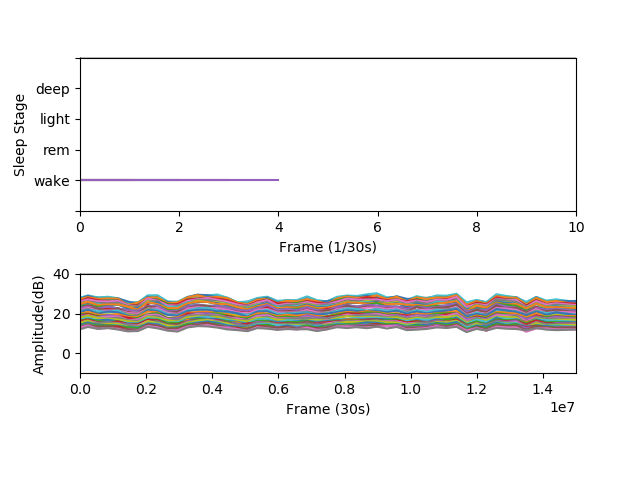
\includegraphics[width=70mm,scale=0.2]{VIS05.png}}
		\caption{An example of data collection with Wake Stage.}
		\label{fig:dataCollect01}
	\end{figure}
	\begin{figure}[htbp]
		\centerline{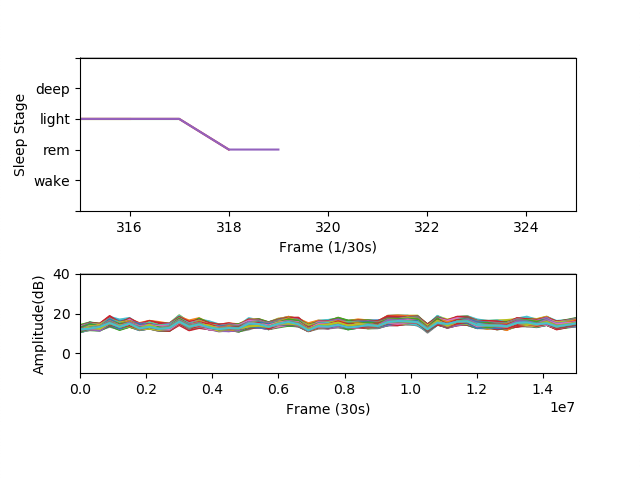
\includegraphics[width=70mm,scale=0.2]{VIS06.png}}
		\caption{An example of data collection with REM Stage.}
		\label{fig:dataCollect02}
	\end{figure}
	\begin{figure}[htbp]
		\centerline{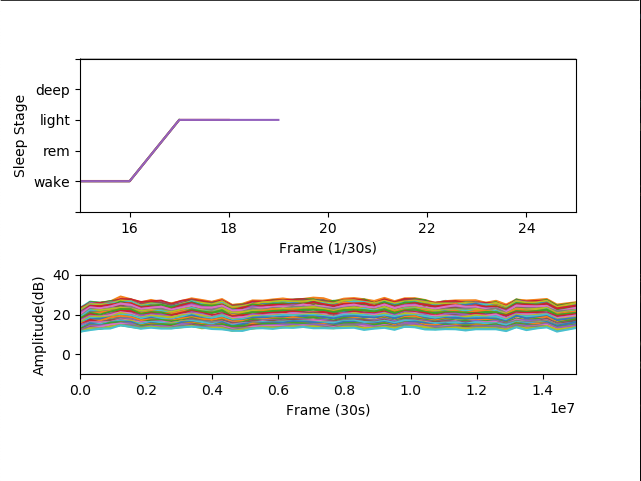
\includegraphics[width=70mm,scale=0.2]{VIS07.png}}
		\caption{An example of data collection with Light Stage.}
		\label{fig:dataCollect03}
	\end{figure}
	\begin{figure}[htbp]
		\centerline{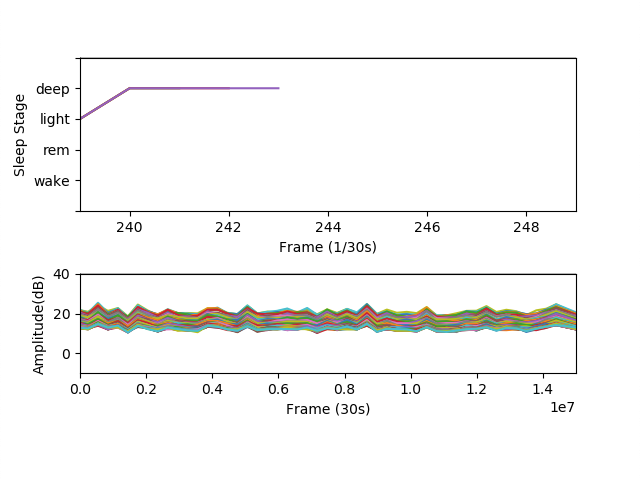
\includegraphics[width=70mm,scale=0.2]{VIS08.png}}
		\caption{An example of data collection with Deep Stage.}
		\label{fig:dataCollect04}
	\end{figure}
	
	The whole data collection is  50 hours of sleep which worth 6,000 frames for 30 seconds/Sleep State rate. The ratio of dataset for training and testing is 85/15.
	
	\subsection*{Experimental Result}
	\label{result}	
	
	An evaluation is achieved   by the algorithm written in Python 3.8. The code is available on Github$\footnote[1]{https://github.com/rtmtree/CSPS}$.
	
	As parameters stated in the previous sections, we demostrated the prediction by the followings.
	
	Table~\ref{table:resultSigma1}, Table~\ref{table:resultSigma2}, Table~\ref{table:resultSigma3} and  Table~\ref{table:resultSigma4} show the estimation performance of 4 Sleep Stages when $\delta=15$, $\delta=30$, $\delta=50$ and $\delta=200$ respectively.
	\begin{table}[!ht]
		\begin{adjustwidth}{-2.25in}{0in} % Comment out/remove adjustwidth environment if table fits in text column.
			\centering
			\caption{
				{\bf Table of evaluation result when $\delta=15$.}}
			\begin{tabular}{l|llllll}
				\backslashbox{Truth}{Predicted} &Wake & REM &Light &Deep \\[1pt]
				\hline
				Wake &0.19 & 0.06 & 0.72 & 0.03 \\[1pt]
				REM &0.03 & 0.83 & 0.14 & 0.00 \\[1pt]
				Light &0.01 & 0.05 & 0.91 & 0.03 \\[1pt]
				Deep &0.00 & 0.01 & 0.16 & 0.83 \\[1pt]
			\end{tabular}
			\label{table:resultSigma1}
		\end{adjustwidth}
	\end{table}
	
	\begin{table}[!ht]
		\begin{adjustwidth}{-2.25in}{0in} % Comment out/remove adjustwidth environment if table fits in text column.
			\centering
			\caption{
				{\bf Table of evaluation result when $\delta=30$.}}
			\begin{tabular}{l|llllll}
				\backslashbox{Truth}{Predicted} &Wake & REM &Light &Deep \\[1pt]
				\hline
				Wake &0.28 & 0.16 & 0.50 & 0.06 \\[1pt]
				REM &0.00 & 0.82 & 0.18 & 0.00 \\[1pt]
				Light &0.01 & 0.04 & 0.92 & 0.03 \\[1pt]
				Deep &0.01 & 0.00 & 0.20 & 0.79 \\[1pt]
			\end{tabular}
			\label{table:resultSigma2}
		\end{adjustwidth}
	\end{table}
	
	\begin{table}[!ht]
		\begin{adjustwidth}{-2.25in}{0in} % Comment out/remove adjustwidth environment if table fits in text column.
			\centering
			\caption{
				{\bf Table of evaluation result when $\delta=50$.}}
			\begin{tabular}{l|llllll}
				\backslashbox{Truth}{Predicted} &Wake & REM &Light &Deep \\[1pt]
				\hline
				Wake &0.34 &0.06 &0.5 & 0.09 \\[1pt]
				REM &0.00 & 0.83 & 0.17 & 0.00 \\[1pt]
				Light & 0.01 & 0.03 & 0.92 & 0.04 \\[1pt]
				Deep &0.01 & 0.00 & 0.15 & 0.85 \\[1pt]
			\end{tabular}
			\label{table:resultSigma3}
		\end{adjustwidth}
	\end{table}
	
	\begin{table}[!ht]
		\begin{adjustwidth}{-2.25in}{0in} % Comment out/remove adjustwidth environment if table fits in text column.
			\centering
			\caption{
				{\bf Table of evaluation result when $\delta=200$.}}
			\begin{tabular}{l|llllll}
				\backslashbox{Truth}{Predicted} &Wake & REM &Light &Deep \\[1pt]
				\hline
				Wake &0.19 & 0.06 & 0.66 & 0.09 \\[1pt]
				REM &0.03 & 0.76 & 0.21 & 0.00 \\[1pt]
				Light &0.01 & 0.04 & 0.91 & 0.04 \\[1pt]
				Deep &0.01 & 0.00 & 0.17 & 0.82 \\[1pt]
			\end{tabular}
			\label{table:resultSigma4}
		\end{adjustwidth}
	\end{table}
	
	\section*{Discussion}
	
	\subsection*{Environment Installation}
	
	The Installation of WiFi antennae can affect tremendously in data. We fixed the positions in both training and testing process as shown in Fig.~\ref{fig:SETUP01}.
	2 antennae are connecting to ESP32s and to the PC afterward for the AP antennae for CSI collection. Lastly, the human sleeping on the bed need to wear Fitbit sleep tracker as shown in Fig.~\ref{fig:SETUP02}.
	
	\begin{figure}[htbp]
		\centerline{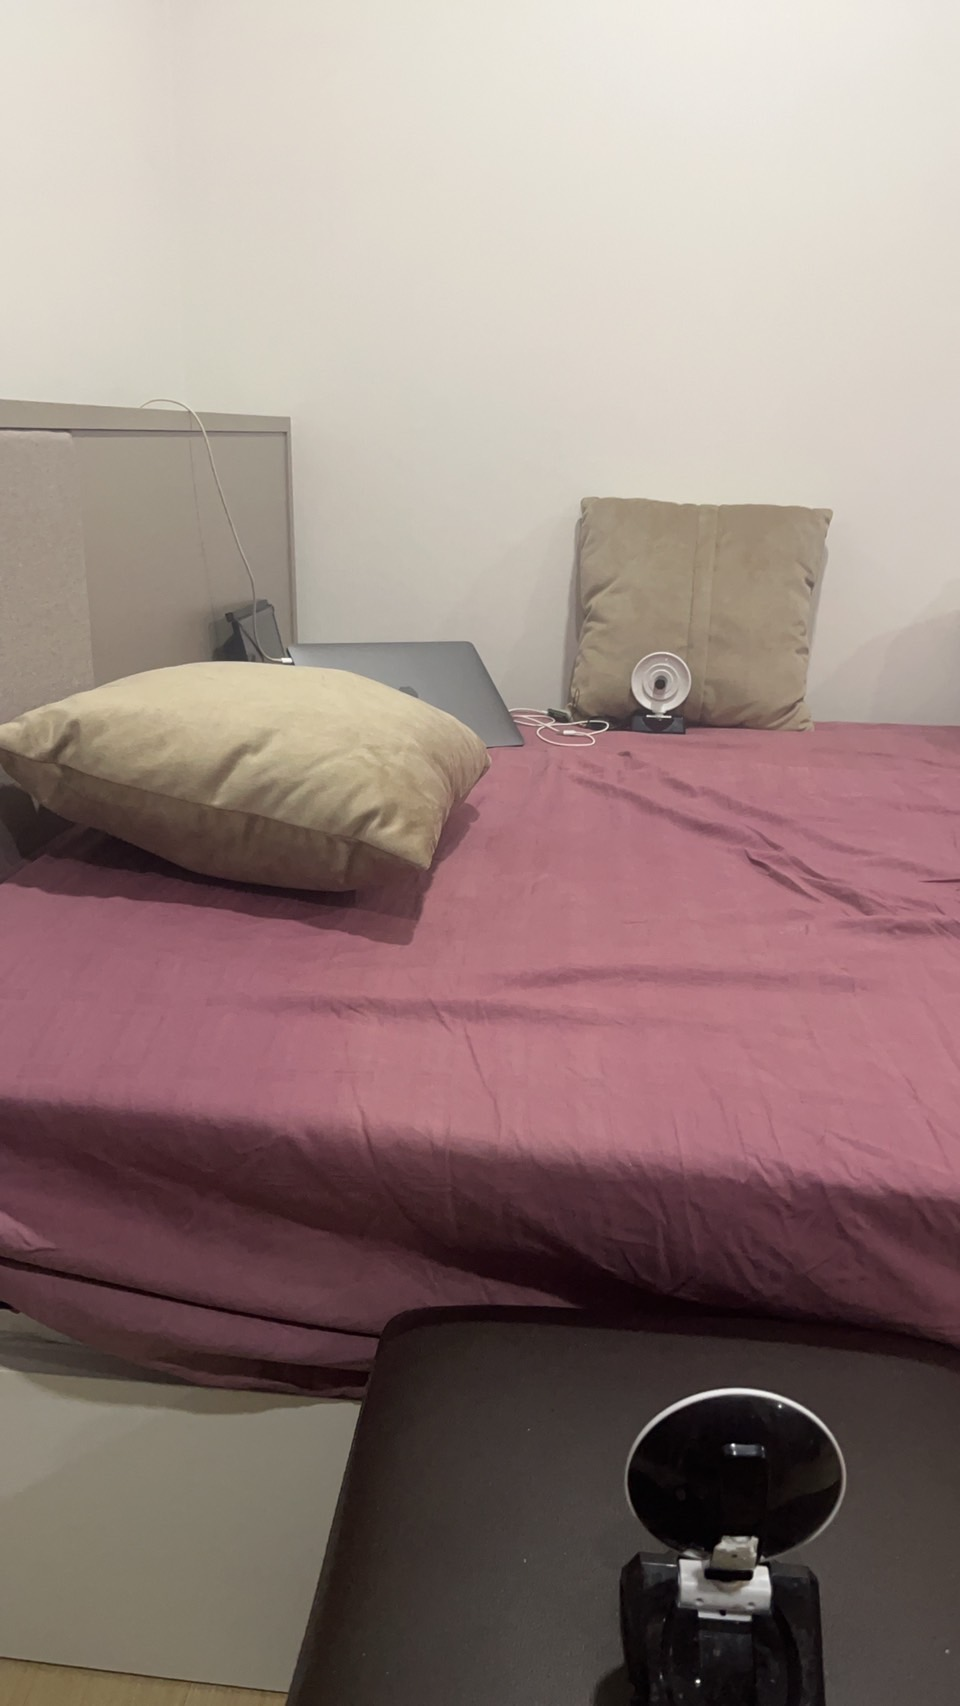
\includegraphics[width=40mm,scale=0.2]{SETUP01.jpg}}
		\caption{Camera setup and a bed.}
		\label{fig:SETUP01}
	\end{figure}
	
		\begin{figure}[htbp]
		\centerline{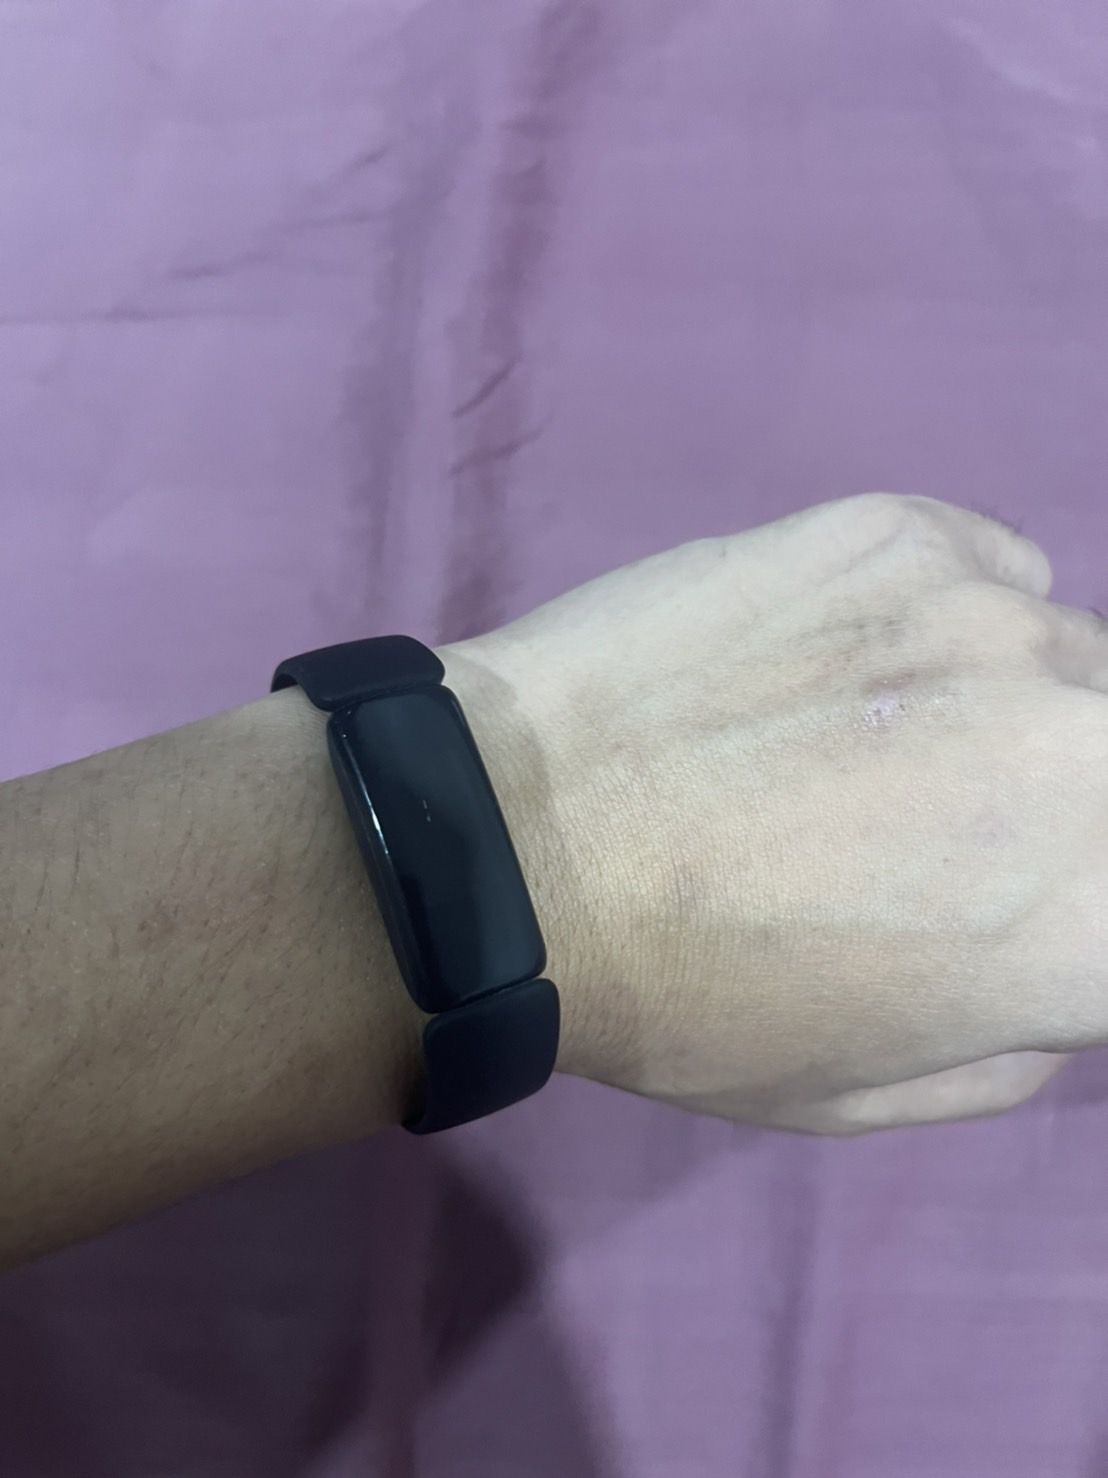
\includegraphics[width=40mm,scale=0.2]{SETUP03.jpg}}
		\caption{Fitbit sleep tracker.}
		\label{fig:SETUP02}
	\end{figure}
	
	
	
	\subsection*{CSI Extraction Method}
	
	There are many solutions for extracting WiFi CSI from the ESP32 as mentioned in \nameref{ESP32}. This paper picked the solution from ESP32-CSI-Tool$\footnote[1]{https://github.com/StevenMHernandez/ESP32-CSI-Tool}$ since it is considerably well-written and simple to organize. To change the method of extracting WiFi CSI would affect the result significantly.
	
	
	
	\subsection*{Multiple Person Sleep Stage Estimation}
	
	The model does a mapping rule from WiFi CSI with a specific dimension to human sleep stage matrix. So, it is able to only detect single person pose in a range. The annotations originally can result all human sleep stage by using the devices for all specimen. If we do training with multiple sleep stage data instead, we do not believe the result will be well since CSI of a person moving is rarely separatable form others.
	
	\iffalse
	\subsection*{Human speed of moving to $\sigma$}
	
	As the Table~\ref{table:PCKsigma15}, Table~\ref{table:PCKsigma20}, Table~\ref{table:PCKsigma30} and  Table~\ref{table:PCKsigma40} show the difference of quality by different value of $\sigma$, the fine-tuning says that $\sigma=15$ result the best. This implies length of $15$ frames can represent a specific pattern of move best for the used dataset. So, the volunteer who recorded movement in the datasent perform a move slower, $\sigma$ should be extended to cover the proper time peroid of the movement pattern.
	\fi
	
	\section*{Conclusion}
	
	\iffalse
	Currently, there are many issues on security occuring in all ranges of human especially in elderlies and those who are not capable to live solely. To solve those, issues on privacy usually comes instead e.g. recording videos for preventing accident in a house, monitoring of people in a room. Many people do not feel very comfortable on these. So, we seek a solution where we can monitor those activity without a camera needed. 
	\fi
	Currently, there are many concern on sleepness in all group of people. Especially, those who works in extraordinary time period are facing problem of having deficient sleepness. They are pleased to pay for a device that can inform if their sleepness is well enough e.g. smartwatch, smart ring and smart mattress. Those options come with additional and uncomfortable since users' bodies need a contact to an external device. So, we aim for proposing a contactless Sleep Monitoring device.
	
	After having a research, we discoverd that a variation in WiFi called WiFi CSI can tell whether the area is having an activity or moving objects. Moreoever, \cite{chowdhuryTZ}, \cite{zouH} and many other works had been done very well on detecting even what kind of activities is happening in the area. We do not believe that this is the limitation of WiFi CSI. In order to solve the above problem and prove if WiFi CSI is precise enough, we tried to overcome this by extracting a deeper information like Sleep Stage Estimation from it. 
	
	We controlled environments and enhanced WiFi antennae stability as much as possible then mapped it to the Sleep Stage annotated by Fitbit technology. The result was very poor since the WiFi CSI is very vague. It penetrates through most of the things. We learned from \cite{bib20} that WiFi CSI value does not matter than its change. The works used Long-short term memory (LSTM), a neural network where focusing on sequence of the data, and obtained a very good result.  
	
	We applied the idea of LSTM instead and obtained a lot better result with more than 80\% of overall accuracy. Then, we adjusted the model to be suitable for our type of data and did fine-tuning for the frame size to be fit the most for normal human speed of moving while sleeping. So, This paper proposed a model of mapping rule that can takes a sequence of 30-second WiFi circumstance as an input and return an according human sleep stage as an output. The work can help people to monitor Sleep Stage of elderlies and those who are in need of sleep concerning. Moreover as a contact is not needed, users can not differentiate thier sleeping with or without the device. Significantly, the WiFi CSI obtained from ESP32 which is affordable and widely reachable so, people can simply apply the method on their own. The result of various fine-tuned environments and parammeters is acceptable and shown in \nameref{result}.
	
	
	\section*{Acknowledgments}
	We thank to Sirindhorn International Institute of Technology for providing technical environment and supportive information.
	
	
	
	\nolinenumbers
	
	% Either type in your references using
	% \begin{thebibliography}{}
		% \bibitem{}
		% Text
		% \end{thebibliography}
	%
	% or
	%
	% Compile your BiBTeX database using our plos2015.bst
	% style file and paste the contents of your .bbl file
	% here. See http://journals.plos.org/plosone/s/latex for 
	% step-by-step instructions.
	% 
	\begin{thebibliography}{10}
		
		\bibitem{bib1}
		Conant GC, Wolfe KH.
		\newblock {{T}urning a hobby into a job: how duplicated genes find new
			functions}.
		\newblock Nat Rev Genet. 2008 Dec;9(12):938--950.
		
		\bibitem{bib2}
		Ohno S.
		\newblock Evolution by gene duplication.
		\newblock London: George Alien \& Unwin Ltd. Berlin, Heidelberg and New York:
		Springer-Verlag.; 1970.
		
		\bibitem{bib3}
		Magwire MM, Bayer F, Webster CL, Cao C, Jiggins FM.
		\newblock {{S}uccessive increases in the resistance of {D}rosophila to viral
			infection through a transposon insertion followed by a {D}uplication}.
		\newblock PLoS Genet. 2011 Oct;7(10):e1002337.
		
		
		
		
		\bibitem{bib4}
		Osokin D.
		\newblock {{R}eal-time 2D Multi-Person Pose Estimation on CPU: Lightweight OpenPose}.
		\newblock arXiv:1811.12004 [cs.CV]. 2018 Nov;18.
		
		\bibitem{bib5}
		Mehta D, Sotnychenko O, Mueller F, Xu W, Sridhar S, Pons-Moll G, Theobalt C.
		\newblock {{S}ingle-Shot Multi-Person 3D Pose Estimation From Monocular RGB}.
		\newblock arXiv:1712.03453 [cs.CV]. 2018 Aug;28.
		
		
		\bibitem{wangF}
		Wang F, Panev S, Ziyi D, Han J, Huang D.
		\newblock {{C}an WiFi Estimate Person Pose?}.
		\newblock arXiv:1904.00277 [cs.CV]. 2019 Apr;2.
		
		
		
		\bibitem{liuJ}
		Liu J, Liu H, Chen Y, Wang Y, Wang C.
		\newblock {{W}ireless Sensing for Human Activity: A Survey}.
		\newblock IEEE COMMUNICATIONS SURVEYS \& TUTORIALS, VOL. 22, NO. 3, THIRD QUARTER 2020.
		
		\bibitem{chowdhuryTZ}
		Chowdhury TZ, Leung C, Miao CY.
		\newblock {{W}iHACS: Leveraging WiFi for Human Activity Classification using OFDM Subcarriers’ correlation}.
		\newblock IEEE, GlobalSIP 2017.
		
		
		\bibitem{bib9}
		Guo L, Wang L, Liu J, Zhou W, Lu B.
		\newblock {{H}uAc: Human Activity Recognition Using Crowdsourced WiFi
			Signals and Skeleton Data}.
		\newblock Wireless Communications and Mobile Computing
		Volume 2018, Article ID 6163475.
		
		
		
		\bibitem{bib10}
		Wang F, Feng J, Zhao Y, Xiaobin Zhang, Zhang S.
		\newblock {{J}oint Activity Recognition and Indoor
			Localization with WiFi Fingerprints}.
		\newblock arXiv:1904.04964 [cs.CV]. 2019 Jul;18.
		
		
		\bibitem{bib11}
		Al-qaness MAA, Li F, Ma X, Zhang Y, Liu G.
		\newblock {Device-Free Indoor Activity Recognition System}.
		\newblock Appl. Sci. 2016, 6, 329; doi:10.3390.
		
		\bibitem{bib12}
		Wang W, Liu AX, Shahzad M, Ling K, Lu S.
		\newblock {{D}evice-free Human Activity Recognition Using Commercial WiFi Devices}.
		\newblock  IEEE Journal
		on Selected Areas in Communications. DOI 10.1109/JSAC.2017.2679658.
		
		\bibitem{bib13}
		Zhao T, Li F, Tian P.
		\newblock {{A} Deep-Learning Method for Device Activity Detection in mMTC Under Imperfect CSI Based on Variational-Autoencoder}.
		\newblock IEEE TRANSACTIONS ON VEHICULAR TECHNOLOGY, VOL. 69, NO. 7, JULY 2020.
		
		\bibitem{bib14}
		Liu J, Teng G, Hong F.
		\newblock {{H}uman Activity Sensing with Wireless Signals: A Survey}.
		\newblock Sensors 2020, 20, 1210; doi:10.3390/s20041210.
		
		\bibitem{bib15}
		Yousefi S, Narui H, Dayal S, Ermon S, Valaee S.
		\newblock {{A} Survey on Behaviour Recognition Using WiFi Channel State Information}.
		\newblock arXiv:1708.07129 [cs.AI]. 2017 Aug;23.
		
		\bibitem{bib16}
		Chen Z, Zhang L, Jiang C, Cao Z, Cui W.
		\newblock {{W}iFi CSI Based Passive Human Activity Recognition Using Attention Based BLSTM}.
		\newblock  IEEE TRANSACTIONS ON MOBILE COMPUTING, VOL. 18, NO. 11, 2019 Nov.
		
		\bibitem{bib17}
		Li B, Cui W, Wang W, Zhang L, Chen Z, Wu M.
		\newblock {{T}wo-Stream Convolution Augmented Transformer for Human Activity Recognition}.
		\newblock Association for the Advancement of Artificial
		Intelligence, 2021.
		
		\bibitem{bib18}
		Luo Y, Ren J, Wang Z, Sun W, Pan J, Liu J, Pan J, Lin L.
		\newblock {{L}STM Pose Machines}.
		\newblock arXiv:1712.06316 [cs.CV].
		
		\bibitem{bib19}
		Lee K, Lee I, Lee S.
		\newblock {{P}ropagating LSTM: 3D Pose Estimation based on Joint Interdependency}.
		\newblock Computer Vision – ECCV 2018. ECCV 2018. Lecture Notes in Computer Science, vol 11211. Springer, Cham.
		
		\bibitem{bib20}
		Du X, Vasudevan R, Johnson-Roberson M.
		\newblock {{B}io-LSTM: A Biomechanically Inspired Recurrent Neural Network for 3D Pedestrian Pose and Gait Prediction}.
		\newblock arXiv:1809.03705 [cs.RO]. 2019 Sep;13.
		
		\bibitem{bib21}
		Hossain MRI, Little JJ.
		\newblock {{E}xploiting temporal information for 3D human pose estimation}.
		\newblock arXiv:1711.08585 [cs.CV]. 2018 Sep;12.
		
		\bibitem{bib22}
		Pavllo D, Feichtenhofer C, Grangier D, Auli M.
		\newblock {{3}D human pose estimation in video with temporal convolutions and semi-supervised training}.
		\newblock arXiv:1811.11742 [cs.CV]. 2019 Mar;29.
		
		\bibitem{bib23}
		Chen T, Fang C, Shen X, Zhu Y, Chen Z, Luo J.
		\newblock {{A}natomy-aware 3D Human Pose Estimation with Bone-based Pose Decomposition}.
		\newblock arXiv:2002.10322 [cs.CV]. 2021 Jan;26.
		
		\bibitem{bib24}
		Ruiz AH, Porzi L, Bulo SR, Moreno-Noguer F.
		\newblock {{3}D CNNs on Distance Matrices for Human Action Recognition}.
		\newblock MM ’17, Mountain View, CA, USA. 2017 Oct;23–27.
		
		
		\bibitem{hernandezSM}
		Hernandez SM, Bulut E.
		\newblock {{L}ightweight and Standalone IoT based WiFi Sensing for Active Repositioning and Mobility.}
		\newblock IEEE 21st International Symposium on ``A World of Wireless, Mobile and Multimedia Networks" (WoWMoM), 2020.
		
		\bibitem{atifM}
		Atif M, Muralidharan S, Ko H, Yoo B.
		\newblock {{W}i-ESP—A tool for CSI-based Device-Free Wi-Fi Sensing (DFWS).}
		\newblock Journal of Computational Design and Engineering, 2020, 7(5), 644–656.
		
		\bibitem{zouH}
		Zou H, Zhou Y, Yang J, Jiang H, Xie L, Spanos CJ.
		\newblock {{D}eepSense: Device-free Human Activity Recognition via Autoencoder Long-term Recurrent Convolutional Network.}
		\newblock 2018 IEEE International Conference on Communications (ICC), Kansas City, MO, USA, 2018, pp. 1-6, doi: 10.1109/ICC.2018.8422895.
		
		\bibitem{hochreiterS}
		Hochreiter S, Schmidhuber J.
		\newblock {{L}ONG SHORT-TERM MEMORY.}
		\newblock Neural Computation 9(8):1735-1780, 1997.
		
		
		
		
	\end{thebibliography}
	
	
	
\end{document}

